\chapter{Introduzione}
\label{chap:chap1}
% OTTIMIZZAZIONE DEL PATH TRACKING CON MODEL PREDICTIVE CONTROL PER AUTONOMOUS RACING NEL CONTESTO DI F1TENTH
% Presentare il lavoro svolto e gli obiettivi da raggiungere
Nell'ultimo decennio il settore della guida autonoma ha fatto grandi progressi grazie
all'introduzione di nuovi algoritmi e tecniche avanzate nel campo della robotica e 
dell'intelligenza artificiale. L'\textit{autonomous driving} rappresenta una sfida
tecnologica molto complessa poiché è caratterizzata da diversi ambiti di ricerca, quali 
percezione, pianificazione e controllo.
In aggiunta alle più classiche applicazioni di guida autonoma, come il trasporto
pubblico urbano e le automobili con funzionalità di guida assistita o totalmente autonoma,
un settore altamente competitivo che sta attirando sempre più attenzione è quello 
dell'\textit{autonomous racing}. Le auto da corsa possono essere veicoli reali -- come 
una vettura di \textit{Formula 1} -- o veicoli a scala ridotta -- ad esempio scala 1:10 per \textit{F1TENTH}.
Proprio comunità come quella di \textit{F1TENTH} stanno raggiungendo ottimi risultati grazie a delle vere e
proprie competizioni, che permettono di far gareggiare ingegneri e ricercatori provenienti
da tutto il mondo con veicoli autonomi in condizioni estreme, mettendo alla prova le 
prestazioni delle proprie soluzioni in ambienti a velocità elevate, come dei circuiti.
I partecipanti possono così affrontare le sfide del controllo più estreme in un 
ambiente controllato, riflettendo però le dinamiche del mondo reale.

A differenza della guida su strada, lo scopo è quello di guidare in sicurezza nel modo
più veloce ed efficiente, riducendo i tempi di completamento su piste competitive. 
In questo contesto, vi sono dunque due sfide cruciali: la pianificazione della traiettoria e sistemi di controllo robusti e accurati, in grado di gestire variazioni improvvise.
Inoltre, il controllo del veicolo ha il compito di ottimizzare il percorso seguito e di minimizzare gli errori di traiettoria. 
%Metodi reattivi come \textit{Pure Pursuit} e \textit{PID Controller} sono stati ampiamente usati fino a un certo punto, ma di recente metodi più sofisticati, come il Model Predictive Control (MPC), hanno mostrato un enorme potenziale.

L'obiettivo del lavoro di tesi è sviluppare e analizzare l'efficacia di 
\textit{Model Predictive Control (MPC)}, un metodo di controllo avanzato per 
l'ottimizzazione dell'attività di \textit{path tracking}, applicata in un
contesto di \textit{autonomous racing} su veicoli in scala 1:10 per la piattaforma
\textit{F1TENTH}.
Attraverso l'implementazione dell'algoritmo e la simulazione su diversi tracciati di 
\textit{Formula 1}, si confrontano le prestazioni di \textit{MPC} con quelle di 
\textit{Pure Pursuit}, un altro algoritmo di controllo più semplice basato su 
\textit{metodi reattivi}, secondo diverse metriche individuate.

Il lavoro è stato suddiviso nelle seguenti fasi:
\begin{description}
\item[Capitolo 1: Introduzione] Si fornisce una panoramica di \textit{F1TENTH} e del 
contesto dell'\textit{autonomous racing}. In seguito, si introducono i concetti 
chiave di \textit{ROS}, alla base di tutta l'implementazione del progetto.
\item[Capitolo 2: Metodi reattivi per il controllo] Si discutono i metodi di controllo 
reattivi, come il \textit{PID Controller}, individuando vantaggi e limitazioni di queste
soluzioni per il contesto trattato.
\item[Capitolo 3: Model Predictive Control] Si descrive l'algoritmo oggetto di questa 
tesi, trattandone la struttura, l'\textit{orizzonte}, il modello utilizzato e formulando
il problema di controllo ottimale (obiettivo e vincoli). 
Si discute poi di discretizzazione, linearizzazione e dei vantaggi e svantaggi di questo metodo.
\item[Capitolo 4: Implementazione] Vengono presentati i circuiti utilizzati per mettere alla
prova \textit{MPC} e le sue diverse configurazioni di guida. Dopodiché, si descrive il 
risolutore utilizzato e si discute il codice degli obiettivi e dei vincoli. 
Infine, si approfondisce la fase di \textit{tuning} delle matrici di pesi, fondamentali per l'obiettivo.
\item[Capitolo 5: Analisi dei risultati] Si analizzano i risultati dei profili di \textit{MPC} 
su entrambe le piste, confrontandoli tra loro e con il \textit{Pure Pursuit}.
\item[Capitolo 6: Conclusioni] Si riassumono i principali risultati ottenuti e si
menzionano possibili sviluppi futuri.
\end{description}

%\begin{description}
\section{F1TENTH}
%\lipsum[2]
\textit{F1TENTH} è una comunità internazionale di ricercatori, ingegneri, sviluppatori e appassionati di sistemi autonomi che ogni anno organizza una serie di gare
tra auto autonome da corsa in scala \textit{1:10}, nelle quali squadre provenienti 
da tutto il mondo si riuniscono per competere~\cite{f1tenth}.
Fondata nel 2016 dall'\textit{University of Pennsylvania}, comprende ora diverse università 
provenienti da tutto il mondo, le quali hanno incluso \textit{F1TENTH} nei programmi dei propri 
corsi di laurea, portando a un ulteriore sviluppo della comunità globale.
%\hyperlink{https://f1tenth.org/learn.html}{primo}

\begin{figure}[H]
    \centering
    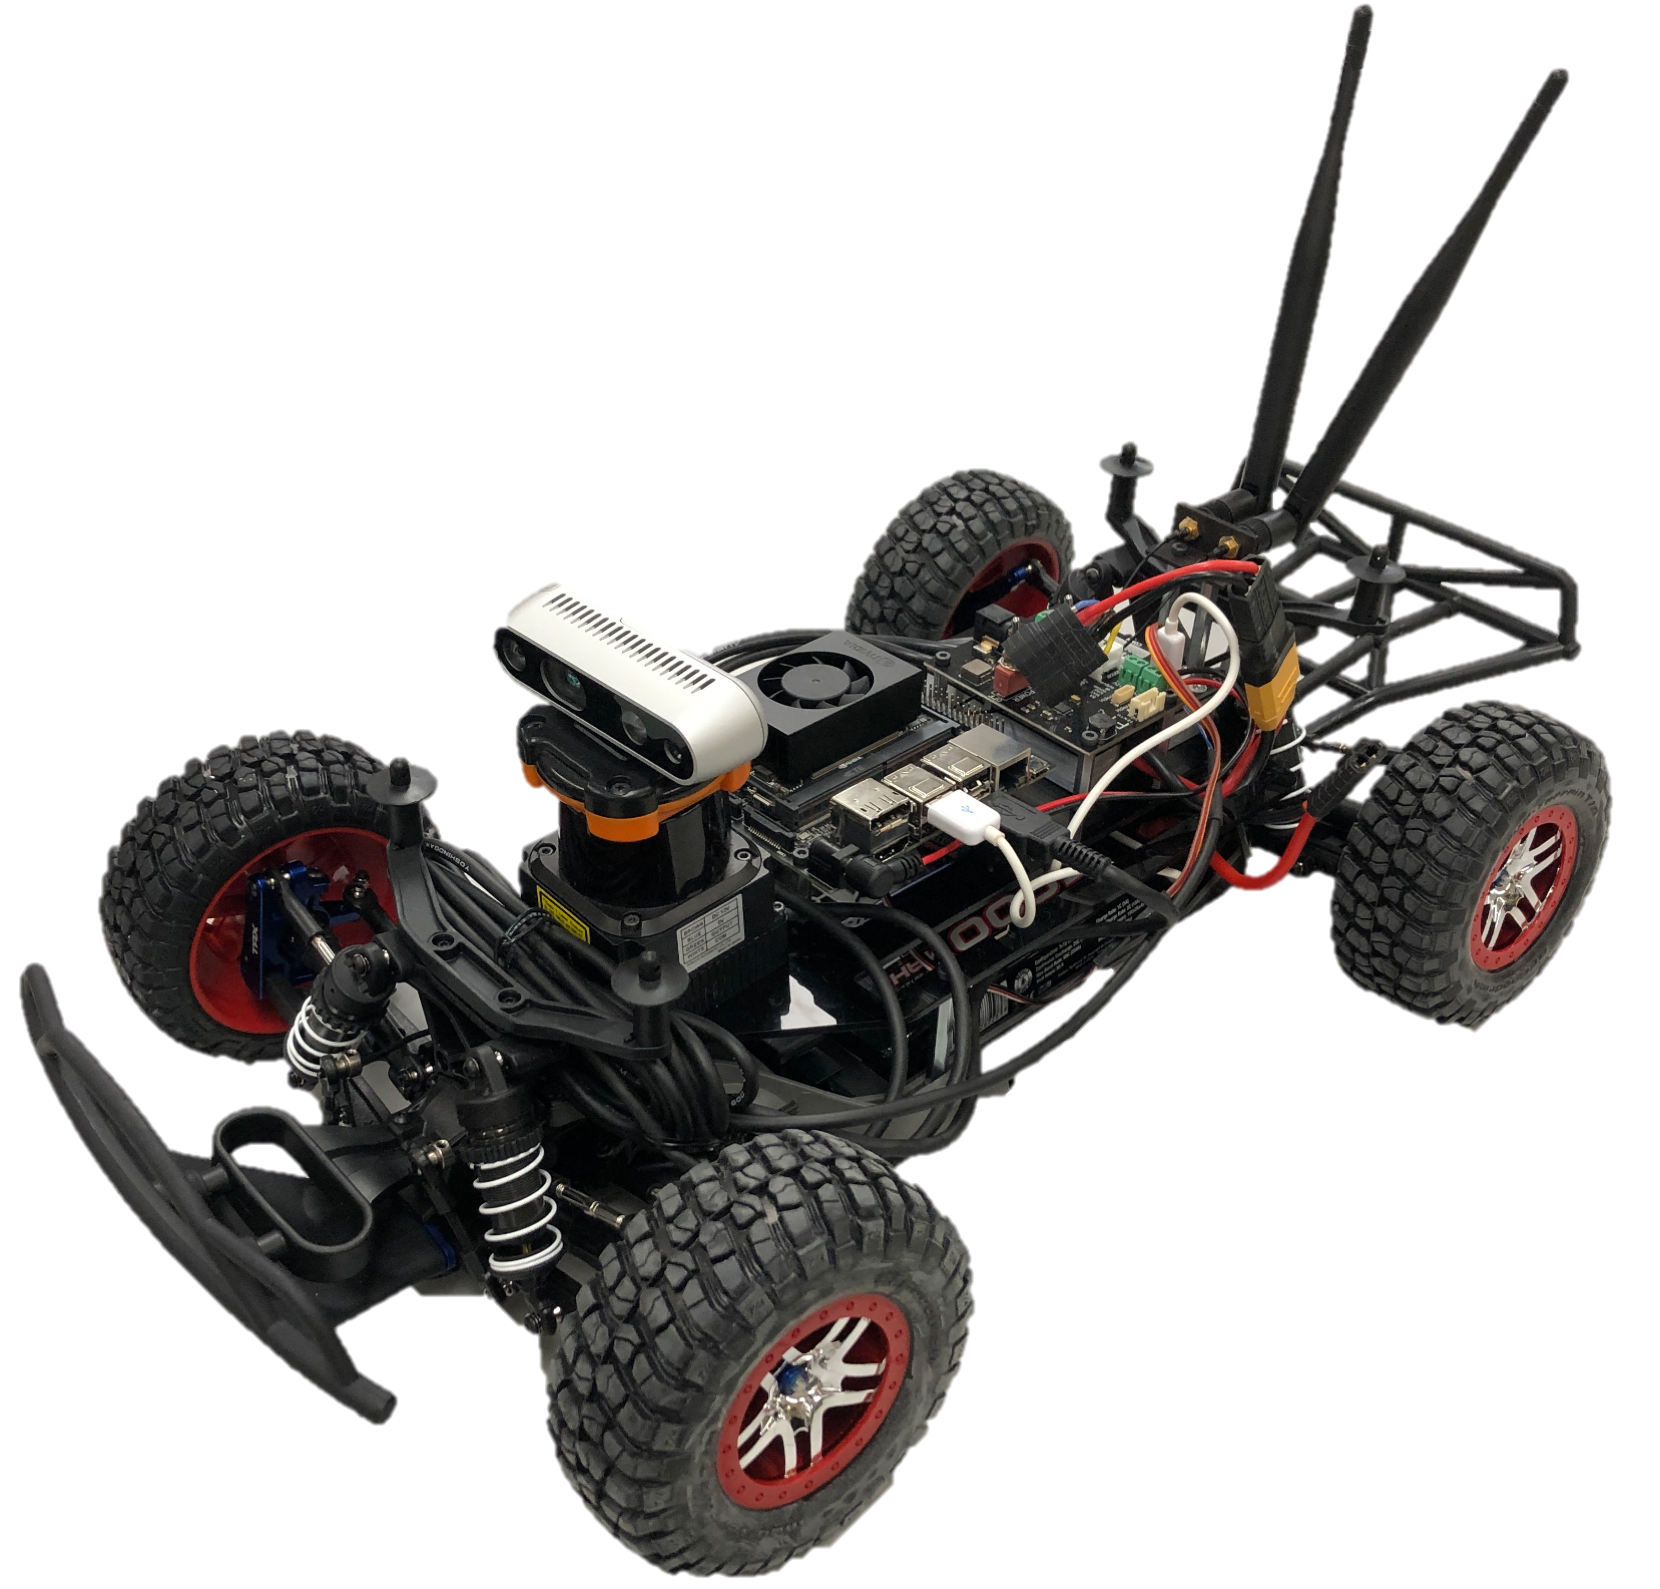
\includegraphics[scale=0.1]{images/F110_car.png}
    \caption{Robot mobile di \textit{F1TENTH} in scala 1:10~\cite{f1tenth}.}
    \label{fig:fig1} % etichetta utilizzata per riferisi all'immagine
\end{figure}

%Oltre alle competizioni, i fondatori hanno organizzato dei corsi gratuiti che insegnano
%i fondamenti della guida autonoma, introducendo gli studenti all'hardware, al software
%e agli algoritmi coinvolti nella costruzione e nello sviluppo di un'auto a guida autonoma. 
%Questi corsi incentivano 
La piattaforma di sviluppo di \textit{F1TENTH} incentiva lo studio e la ricerca nelle 
discipline della guida autonoma, della robotica e dell'intelligenza artificiale; inoltre, essa 
permette di andare a sviluppare anche le capacità analitiche necessarie per ragionare su 
situazioni etiche nella fase di progettazione dei propri veicoli autonomi.

L'obiettivo degli organizzatori consiste quindi nel fornire le basi sulle più
recenti tecnologie implementate e testate sulle auto a guida autonoma e, più in generale, sui sistemi mobili autonomi.
\begin{figure}[H]
    \centering
    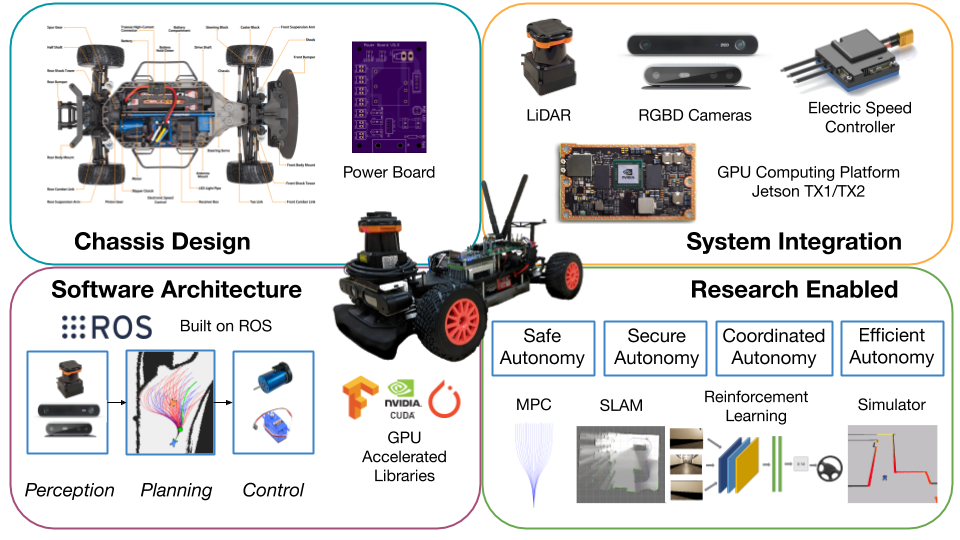
\includegraphics[width=\textwidth]{images/F110_architecture.png}
    \caption{Stack architetturale di \textit{F1TENTH}~\cite{learnf1tenth}.}
    \label{fig:fig2} % etichetta utilizzata per riferisi all'immagine
\end{figure}
\noindent In primo luogo, è stato effettuato uno studio preliminare della piattaforma F1TENTH e dei concetti 
fondamentali della guida autonoma. Essi comprendono le seguenti macro-aree tematiche:
\begin{itemize}
    \item Infrastruttura di \textit{ROS 2} e il simulatore \textit{F1TENTH Gym};
    \item Dinamica del veicolo e \textit{metodi reattivi} -- Comprende la modellazione e la 
    simulazione della dinamica del veicolo, i metodi
    di navigazione reattiva, come l'algoritmo 
    \textit{PID} applicato al \textit{Wall Following} e l'algoritmo \textit{Follow the Gap} per evitare gli ostacoli.
    \item \textit{Mapping} e \textit{Localization} -- Concetti come la stima dello stato, la 
    modellazione dell'ambiente, le tecniche basate su filtri per la localizzazione del robot e la tecnica \textit{SLAM}.
    \item \textit{Control} e \textit{Planning} -- Tematiche fondamentali per la progettazione di 
    veicoli a guida autonoma, come il \textit{path tracking} con \textit{Pure Pursuit}
    e gli algoritmi di pianificazione del movimento di un robot, come \textit{RRT}, 
    altri metodi basati su \textit{spline} o \textit{clotoidi} e altri tipi di \textit{planner}.
\end{itemize}
Inoltre, durante questa fase iniziale sono stati implementati, mediante
\textit{Python} e le relative librerie per ROS 2, i seguenti algoritmi:
\begin{enumerate}
    \item \textit{Frenata di emergenza automatica}: si calcola il tempo istantaneo alla
    collisione (\textit{iTTC}) grazie al messaggio \verb|LaserScan| nel simulatore, al cui 
    interno è presente un array che contiene tutte le misurazioni del LiDAR.
    \item \textit{Wall Following}: si è implementato un \textit{controller PID} per 
    far correre l'auto parallelamente alle pareti di un corridoio ad una distanza fissa;
    \item \textit{Follow the Gap}: si tratta di un algoritmo \textit{reattivo}
    per evitare gli ostacoli che permette al robot di percorrere più giri all'interno della mappa utilizzata;
    \item \textit{Pure Pursuit}: è stato utilizzato \textit{SLAM} per effettuare il \textit{mapping}
    e, al contempo, la localizzazione del veicolo. Il \textit{mapping} è il processo di 
    creazione di una rappresentazione dell'ambiente circostante, mentre la \textit{localizzazione} 
    consiste nel determinare la posizione dell'auto rispetto alla mappa. Invece, per ottenere la 
    localizzazione a partire dalla mappa generata, è stato impiegato un \textit{Particle Filter}. 
    È stato così possibile implementare l'algoritmo \textit{Pure Pursuit}, nel quale viene calcolata 
    iterativamente la curvatura dell'arco da seguire. Questo metodo, infatti, permette di seguire una 
    traiettoria composta da più punti (\textit{waypoint}).
    \item \textit{Motion Planning}: è stata realizzata una struttura per il controllo delle 
    collisioni del veicolo, detta \textit{occupancy grid}. In seguito, è stato implementato 
    l'algoritmo \textit{RRT*} come \textit{local planner} e si è utilizzato \textit{Pure Pursuit}
    come controller.
\end{enumerate}
%Una volta realizzati i laboratori e acquisite le basi necessarie per tutto ciò che riguarda la guida autonoma, si è concentrato lo studio sull'implementazione del Model Predictive Control, che rappresenta l'argomento principale del lavoro di tesi, spiegato nel capitolo 
\section{ROS 2}
Il lavoro oggetto di questa tesi è sviluppato a partire da \textit{Robot Operating System (ROS)}, che consiste in un insieme di librerie software e strumenti
per creare applicazioni robotiche~\cite{doi:10.1126/scirobotics.abm6074}. 
Nato nel 2007, il progetto ha visto numerosi cambiamenti, tra cui il passaggio da
ROS 1 a ROS 2.
Contrariamente a come si potrebbe pensare dal nome, \textit{ROS} non è un sistema 
operativo, bensì si tratta di un \textit{middleware} basato su un meccanismo 
di pubblicazione e sottoscrizione anonimo che consente lo scambio di 
messaggi tra diversi processi.
Un \textit{middleware} è un software che si trova a metà tra un sistema operativo e le
applicazioni in esecuzione al suo interno e permette la comunicazione e la gestione
dei dati per applicazioni distribuite~\cite{middleware}.

Si tratta di un progetto \textit{open source} supportato da una grande comunità di
ricercatori nell'ambito della robotica, i quali effettuano rilasci per più distribuzioni \textit{ROS}. 
Alcune di queste sono dotate di supporto a lungo termine, dunque sono più stabili 
e vengono sottoposte a test approfonditi; rientra in questa categoria \textit{ROS 2 Humble}, 
quella usata per questo lavoro.

\textit{ROS 2} fornisce tutte le funzionalità necessarie per la realizzazione di applicazioni robotiche, 
permettendo dunque di risparmiare più tempo e risorse per sviluppo vero e proprio, una 
caratteristica cruciale, soprattutto, in un contesto lavorativo.
Nello specifico, sono supporti due linguaggi di programmazione: \textit{Python} e \textit{C++}, in base alle proprie conoscenze e/o esigenze.
In questa tesi si è scelto di utilizzare il primo per ogni fase implementativa, come si può
notare al Capitolo \ref{chap:chap4}. Nelle prossime sottosezioni si discute invece 
dei concetti alla base di ROS 2.

\subsection{Nodi}
Un \textit{nodo} rappresenta una singola unità logica che svolge una specifica 
funzione all’interno del processo di esecuzione di un robot. 
Ogni nodo in \textit{ROS} può inviare e ricevere dati da altri nodi tramite 
\textit{topic}, servizi e azioni~\cite{rosdocs}. I nodi possono:
\begin{itemize}
    \item pubblicare su \textit{topic} specifici per fornire dati ad altri nodi;
    \item sottoscriversi per ottenere dati da altri nodi;
    \item agire come un client di servizio per far sì che un altro nodo esegua un 
    calcolo per loro, o come un server di servizio per fornire funzionalità ad altri 
    nodi;
    \item analogamente al servizio, agire come action client/server, per calcoli di 
    lunga durata.
    \item fornire \textit{parametri} per modificare il comportamento 
    durante il runtime.
\end{itemize}

\subsection{Topic}
Un \textit{topic} rappresenta il mezzo di comunicazione tramite cui i nodi si 
scambiano i \textit{messaggi} e risulta particolarmente indicato per flussi di dati 
continui, come quelli dei sensori, lo stato del robot e altre informazioni.

I \textit{messaggi} rappresentano il mezzo con cui un nodo invia dati sulla rete
ad altri nodi, senza alcuna risposta prevista. Questi sono descritti e definiti nei file 
\verb|.msg| nella directory \verb|msg/| di un pacchetto \textit{ROS} e sono composti da 
campi e costanti.

Un \textit{topic} è dunque un sistema di pubblicazione/sottoscrizione \textit{fortemente tipizzato}.
Entrando nello specifico, nel sistema dei topic sono presenti produttori di dati (detti 
\textit{``publishers''}) e consumatori di dati (detti \textit{``subscribers''}). Queste due entità 
sanno come mettersi in contatto tra loro proprio grazie al concetto stesso di \textit{topic}, 
identificato da un nome comune per far sì che le entità possano ``vedersi''.
Quando i dati vengono pubblicati nel \textit{topic} da uno qualsiasi dei \textit{publishers}, 
tutti i \textit{subscribers} attivi nel sistema riceveranno i dati.

Questa struttura ricorda molto il concetto di \textit{bus} nell'informatica, poiché assomiglia 
proprio a quello presente nei dispositivi hardware.
Un'altra peculiarità di \textit{ROS} è che, di fatto, tutto è \textit{anonimo}: questo implica 
che, quando un \textit{subscriber} riceve un dato, generalmente non sa quale 
\textit{publisher} lo abbia originariamente inviato, anche se lo si può scoprire. 
Il vantaggio di questa architettura è che entrambi i soggetti possono essere scambiati a piacimento, senza influenzare il resto del sistema.

\subsection{Parametri e Launch file}
I \textit{parametri} consistono in una coppia \verb|<chiave:valore>| e sono associati ai singoli nodi, in modo da configurarli all’avvio e durante il runtime, senza quindi
dover modificare continuamente il codice.
I valori iniziali dei parametri possono essere impostati durante l'esecuzione del 
nodo tramite argomenti da riga di comando, file \verb|YAML|, o quando si esegue
il nodo, con l'uso di \textit{launch file}.

Un sistema sviluppato con ROS 2 è tipicamente costituito da molti nodi che eseguono 
processi diversi, eventualmente anche su macchine differenti. 
In particolare, i grandi progetti di robotica coinvolgono spesso più nodi
interconnessi, ognuno dei quali può avere a sua volta numerosi parametri.
Sebbene sia possibile eseguire ciascuno di questi nodi separatamente, l'operazione 
si complica rapidamente.

Il sistema dei \textit{launch file} in \textit{ROS 2} ha lo scopo di automatizzare
l'esecuzione di più nodi attraverso l'uso di un unico comando: \verb|ros2 launch <nome_launch_file.py>|. 
La configurazione del file include quali programmi eseguire e quali argomenti passare; 
in pratica, questi file -- scritti in \textit{Python}, \verb|YAML| o \verb|XML| --
consentono di configurare e avviare contemporaneamente più eseguibili contenenti
dei nodi di \textit{ROS}. Durante lo sviluppo di questa tesi, essi si sono rivelati
fondamentali per l'operazione di \textit{``tuning''} degli algoritmi realizzati, come si può notare nella sottosezione~\ref{subs:tuning}).

\section{Simulatore: F1TENTH Gym}
Il simulatore utilizzato per svolgere tutto il lavoro di tesi è \textit{F1TENTH Gym}, 
l'ambiente ufficiale ideato a fini ricerca, in quanto è necessaria una simulazione 
asincrona e realistica dei veicoli, con la possibilità di avere anche più istanze di veicoli 
(\textit{agenti}) nello stesso ambiente.

Il motore fisico del simulatore favorisce la presenza di programmi estremamente paralleli e, 
soprattutto, permette di avere un'esecuzione rapida.
Si specifica che \textit{F1TENTH Gym} è il simulatore alla base di \textit{F1TENTH Gym ROS}, 
un bridge di comunicazione con \textit{ROS 2} per \textit{F1TENTH Gym}, che dunque 
viene trasformato in una simulazione vera e propria per \textit{ROS 2}, visualizzandola nell'applicativo \verb|RViz|.

\begin{figure}[H]
    \centering
    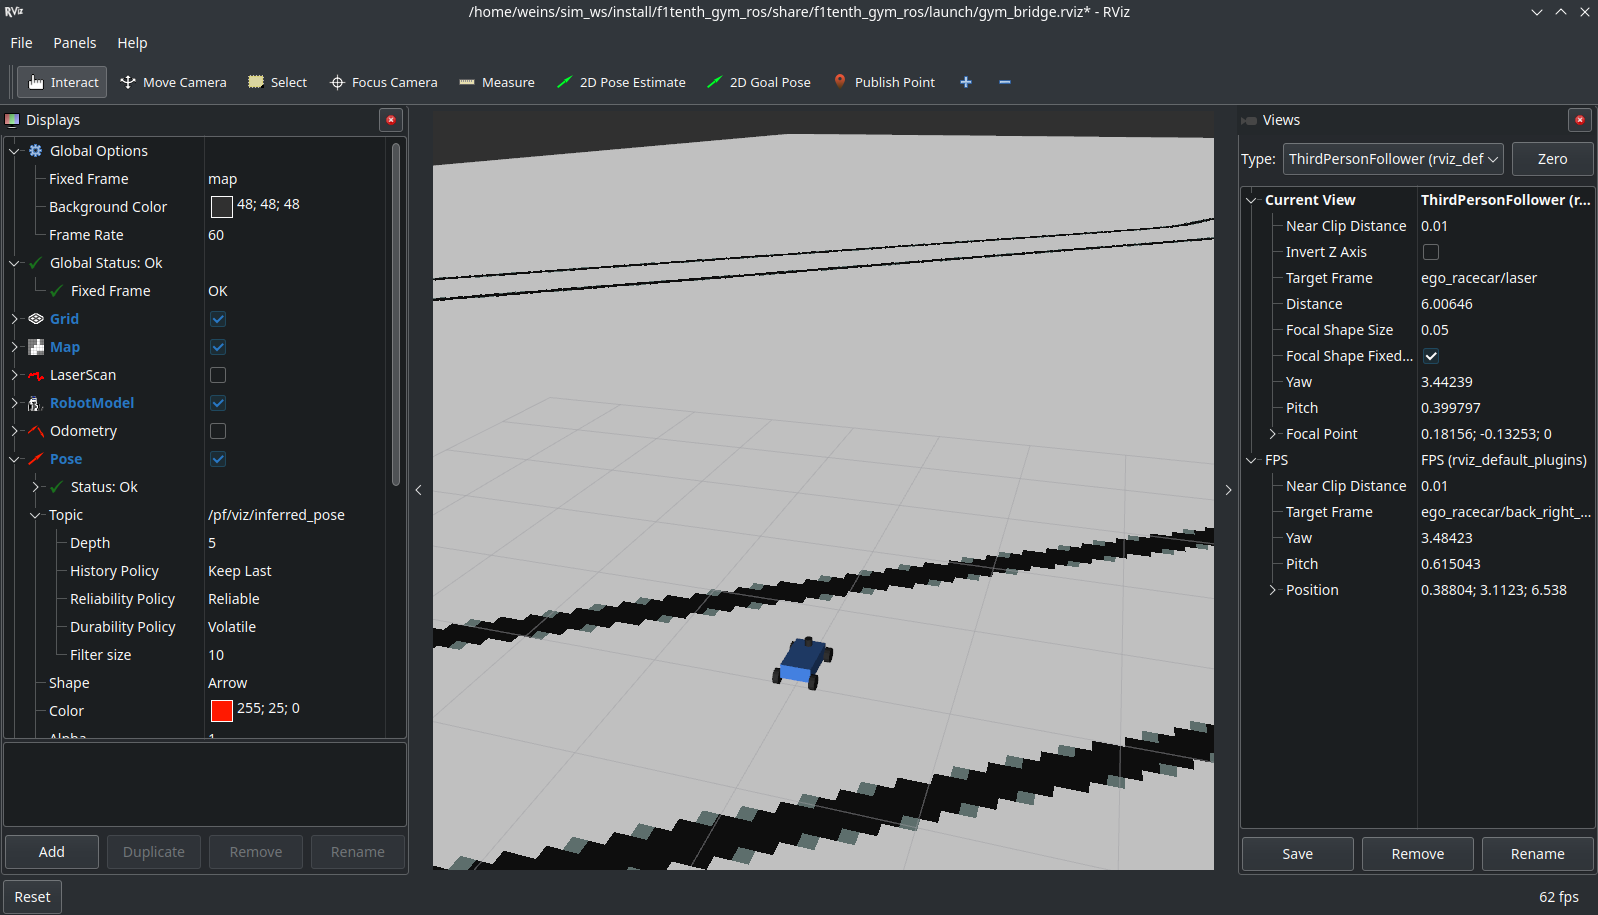
\includegraphics[width=\textwidth]{images/rviz.png}
    \caption{\textit{F1TENTH Gym ROS} con visualizzazione di \textit{RViz}.}
    \label{fig:fig3} % etichetta utilizzata per riferisi all'immagine
\end{figure}

Si specifica che per questo lavoro si è sempre usato un unico agente. Per questa casistica,
i \textit{topic} pubblicati dalla simulazione sono:
\begin{enumerate}
    \item \verb|/scan| -- La scansione laser dell'agente;
    \item \verb|/ego_racecar/odom| -- L'\textit{odometria} dell'agente rappresenta l'uso dei dati provenienti dai sensori di movimento per stimare il cambiamento nel tempo della posizione, dell'orientamento e della velocità.
    \item \verb|/map| -- La mappa dell'ambiente.
\end{enumerate}
Mentre quelli sottoscritti dalla simulazione comprendono:
\begin{enumerate}
    \item \verb|/drive| -- Il comando di guida tramite messaggi \verb|AckermannDriveStamped|.
    \item \verb|/initialpose| -- Permette di reimpostare la posizione dell'agente tramite lo strumento \verb|2D Pose Estimate| di \verb|RViz|.
\end{enumerate}
Anche il nodo \verb|teleop|, relativo al controllo dell'agente con la tastiera, viene incluso come parte della dipendenza del simulatore.

\section{Progettazione dei veicoli a guida autonoma}
La progettazione di veicoli a guida autonoma viene suddivisa in tre macro-aree che
vengono eseguite una dopo l’altra in modo circolare.
% TODO: Spostare sotto la riga di perception

\begin{figure}[h]
    \centering
    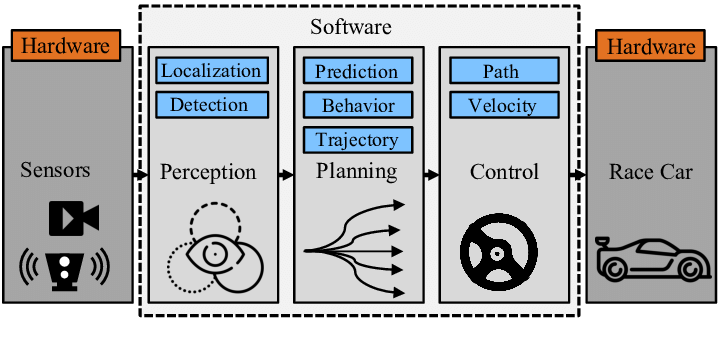
\includegraphics[width=\textwidth]{images/adv_stack.png}
    \caption{Pipeline della guida autonoma~\cite{Betz2022}.}
    \label{fig:fig4} % etichetta utilizzata per riferisi all'immagine
\end{figure}

Ogni area produce degli output utili che vengono passati in input alla 
successiva~\cite{Betz2022}. Dunque, in ordine di esecuzione, il problema è suddiviso in:
\begin{enumerate}
    \item \textit{Perception} -- A partire dai sensori presenti nel robot, costruisce
    un modello dell'ambiente che lo circonda e lo localizza al suo interno.
    \item \textit{Planning} -- Grazie all'output della fase precedente, è in grado
    di determinare il suo stato ed esplorare quelli successivi.
    \item \textit{Control} -- Detto anche \textit{Actuator}, si occupa di generare una 
    sequenza di {input} di sterzata e accelerazione per portare il veicolo allo stato 
    successivo, che è stato generato come output della fase precedente.
\end{enumerate}

Questo ciclo prende anche il nome di \textit{Sense-Plan-Act} e, generalmente, per
garantire una buona performance, lo si vuole completare tra le 20 e 50 volte al secondo.

\subsection{Perception}
La parte di \textit{percezione} comprende la raccolta dei dati dei sensori 
e la successiva elaborazione per avere un \textit{modello} dell'ambiente, proprio
come gli occhi di un guidatore umano.
Di seguito gli obiettivi e le attività svolte da questo modulo applicativo:
\begin{itemize}
    \item \textit{Mapping} -- Si vuole rendere il robot abbastanza intelligente da percepire 
    l’ambiente circostante, così da rilevare ostacoli, altri robot mobili e tutto ciò che lo circonda. 
    \item \textit{Localization} -- Si vuole capire la posizione del robot all’interno
    dell'ambiente. Fondamentalmente, si hanno due tipi di strumenti per ottenere 
    tale conoscenza: le informazioni sull’odometria, fornite dall’\textit{Inertial 
    Measurement Unit (IMU)}, e le informazioni sulle osservazioni,
    fornite dal \textit{LiDAR}.
    \item \textit{Vision} -- Si possono sfruttare metodi classici di visione, come
    \textit{detection} con \textit{OpenCV}, \textit{Visual SLAM}, o metodi basati 
    sul \textit{Deep Learning}, come \textit{Object Detection}. 
    Tuttavia, si specifica che questa tematica non è stata trattata in questo lavoro di tesi.
\end{itemize}
Quando si parla del movimento di un robot mobile bisogna innanzitutto dire che è sempre presente l'incertezza nelle osservazioni; per rappresentare esplicitamente l’incertezza si usa la probabilità, che è alla base dei metodi più comuni per eseguire la localizzazione~\cite{f1tenthcoursel07}, che sono:
\begin{enumerate}
    \item \textit{Bayes Filter}: viene solitamente utilizzato esclusivamente per i casi 
    discreti, cioè con valore finito per lo stato. L’idea alla base è quella di stimare una 
    densità di probabilità nello spazio degli stati condizionata dai dati (percettivi e odometrici).
    \item \textit{Kalman Filter}: algoritmo ricorsivo che utilizza una combinazione di 
    predizioni e misurazioni per stimare lo stato di un sistema nel tempo. Utilizza un metodo 
    basato sui campioni per rappresentare una determinata distribuzione.
    \item \textit{Particle Filter}: chiamato anche \textit{Adaptive Monte Carlo}, si basa su un 
    campionamento pesato e casuale. Si tratta di un \textit{Bayes Filter} ricorsivo,
    simile al \textit{Kalman Filter}, ma ne ``rilassa'' alcune assunzioni. Ogni particella è 
    un’ipotesi di posizione e, invece di campionare ogni volta, ciascun campione viene 
    propagato con il modello di movimento per ottenere i campioni nell’iterazione successiva.
\end{enumerate}

Per il problema di localizzazione, inizialmente si potrebbe pensare di usare 
l'odometria attraverso la tecnica del \textit{dead reckoning}. Si inizia 
cioè da una posizione nota, integrando le misurazioni del controllo e del movimento per stimare la posizione corrente.
Disporre di strumenti o attrezzature migliori sarà senza dubbio di aiuto, tuttavia, esiste
una limitazione fondamentale all’uso della sola odometria: si tratta di un approccio di stima 
\textit{open loop}, dunque non esiste un meccanismo di \textit{feedback} che ci consenta di 
correggere gli errori nella misurazione.
Pertanto, in caso di rumore nelle misurazioni, col passare del tempo si accumulerà l'errore.
Un altro problema correlato è lo slittamento delle ruote, detto \textit{odometry drift}.

La soluzione a queste problematiche è data da \textit{Adaptive Monte Carlo Localization (AMCL)},
un algoritmo di localizzazione basato sul \textit{Particle Filter}~\cite{f1tenthcoursel08}.

\begin{figure}[ht]
    \centering
    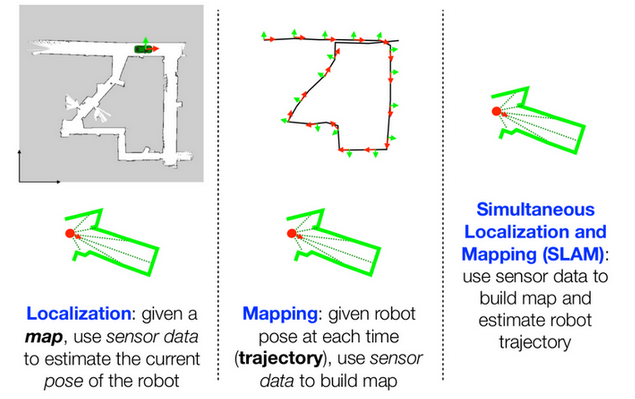
\includegraphics[width=\textwidth]{images/perception.png}
    \caption{Differenza tra localization, mapping e SLAM~\cite{f1tenthcoursel09}.}
    \label{fig:fig5} % etichetta utilizzata per riferisi all'immagine
\end{figure}

\begin{description}
    \item[Problema] -- Per determinare la posizione del robot è necessaria una mappa 
    dell’ambiente, ma si ha prima bisogno della posizione del robot per costruire la mappa stessa.
    \item[Soluzione] -- \textit{Simultaneous Localization and Mapping (SLAM)} è una tecnica che 
    consente ai robot di eseguire simultaneamente la \textit{localizzazione} e il 
    \textit{mapping} di un ambiente sconosciuto. Questo processo continua per diversi istanti 
    di tempo, aggiornando la mappa a ogni passo~\cite{f1tenthcoursel09}.
\end{description}


\subsection{Planning}
\label{subs:planning}
La \textit{pianificazione} consiste nel trovare un percorso ottimo grazie al quale il robot 
possa spostarsi progressivamente dal punto di partenza a quello di \textit{``goal''},
evitando eventuali ostacoli presenti nel cammino.

Generalmente, si suddivide quest'area di sviluppo in una gerarchia di tecniche di \textit{planning}~\cite{f1tenthcoursel12}:
\begin{itemize}
    \item \textit{Global Planner} -- Si tratta di una vista d’insieme del problema per determinare il percorso ottimo;
    \item \textit{Local Planner} -- È una vista che riguarda solo la porzione dell'ambiente 
    vicina al veicolo, sfruttata per individuare le traiettorie possibili per l'auto;
    \item \textit{Behavioral Planner} -- Consiste in una pianificazione delle strategie da 
    adottare in diverse situazioni, selezionando la migliore secondo una specifica funzione di costo.
\end{itemize}

Ad alto livello, le tecniche di pianificazione di un percorso si dividono in due categorie:
\begin{enumerate}
    \item \textit{basate sul campionamento}: \textit{Probabilistic Road Maps (PRM)} e \textit{Rapidly-Exploring Random Tree (RRT*})~\cite{samplingbased};
    \item \textit{basate sulla ricerca}: \textit{A*} e \textit{A* Lattice Planning}.
\end{enumerate}

\subsection{Control}
\label{subs:control}
% Considerare questa img: https://github.com/A-make/awesome-control-theory
Il modulo di \textit{controllo} si occupa dei segnali da inviare agli \textit{attuatori} delle 
ruote (es. angolo di sterzata, freni, ecc.) e del motore (velocità, accelerazione) per portare 
il veicolo al suo stato successivo.

In linea generale, le domande a cui si vuole rispondere sono~\cite{f1tenthcoursel10}:
\begin{itemize}
    \item Come seguire un percorso prestabilito?
    \item Come correggere gli errori di attuazione?
    \item Come guidare il veicolo il più velocemente possibile?
\end{itemize}

Si tratta di un campo di studi così vasto che viene racchiuso nella disciplina 
dell'\textit{ingegneria del controllo}~\cite{f1tenthcoursel04}, che comprende la modellazione 
di una vasta gamma di sistemi dinamici e la progettazione di controllori che garantiscano che 
questi sistemi rispettino il comportamento atteso. In particolare, se ne distinguono due tipologie differenti:
\begin{enumerate}
    \item \textit{Controller Open Loop}: sono adatti per sistemi senza vincoli di dinamica o 
    stabilità, poiché non catturano lo stato del sistema. Inoltre, attuano direttamente la risposta desiderata, senza la continua osservazione dello stato del sistema;
    \item \textit{Controller Closed Loop Feedback}: rispetto ai precedenti, sono indicati per 
    sistemi dinamici e calcolano continuamente un valore di errore $e(t)$, come differenza
    tra la risposta di output desiderata, detta \textit{setpoint}, e una variabile di processo 
    misurata che rappresenta l'output reale.
\end{enumerate}

\begin{figure}[H]
    \centering
    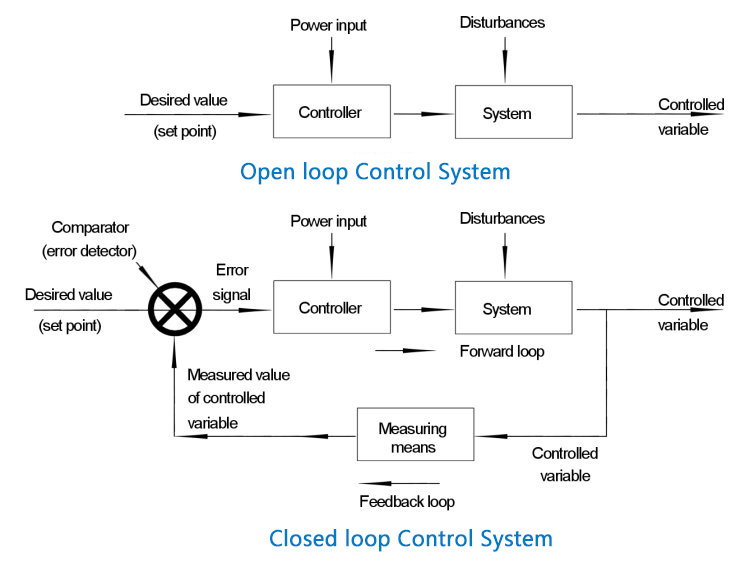
\includegraphics[width=\textwidth]{images/compare_open_closed_loop.jpg}
    \caption{Confronto tra i controller \textit{Open Loop} e \textit{Closed Loop Feedback}~\cite{diffcontrollers}.}
    \label{fig:fig6} % etichetta utilizzata per riferisi all'immagine
\end{figure}

L'obiettivo principale di un controller è quello di applicare automaticamente una 
correzione precisa e reattiva a una certa funzione di controllo, ad esempio, per mantenere
la velocità desiderata, con un ritardo e un superamento minimi, andando ad aumentare gradualmente la potenza del motore.
L’evoluzione del controllo dei veicoli autonomi può essere suddivisa in tre principali fasi di sviluppo~\cite{lect08control}:
\begin{enumerate}
    \item Ispirati dalla comunità della robotica, i primi algoritmi
    di controllo sono stati ispirati da concetti geometrici come la pianificazione di un 
    movimento circolare o l'allineamento del volante verso un percorso \textit{target}. 
    Questi approcci evidenziano buone prestazioni per velocità medio-basse.
    \item All'aumentare delle velocità e delle accelerazioni dei veicoli 
    a guida autonoma, all'interno della comunità di ricerca si sono diffusi più metodi
    di analisi approfonditi, provenienti dalla teoria del controllo e dai sistemi dinamici. 
    Permettono di progettare \textit{controllori state-feedback} e di considerarne più
    effetti dettagliati, come la dinamica dell'imbardata del veicolo e la dinamica dell'attuatore dello sterzo.
    \item Si è in seguito sviluppata una specifica branca del controllo, detta 
    \textit{controllo ottimale}, che vuole controllare un sistema in modo da minimizzare
    o massimizzare un determinato obiettivo. È particolarmente indicata per
    applicazioni complesse: infatti, fa parte di questa classe di problemi il 
    \textit{Model Predictive Control}, il tema principale studiato in questa tesi,
    che verrà discusso nel capitolo~\ref{chap:chap3}.
\end{enumerate}
Gli algoritmi di controllo trattati nel contesto di \textit{F1TENTH} comprendono 
\textit{PID Controller} e \textit{Pure Pursuit}, discussi in dettaglio nel 
Capitolo~\ref{chap:chap2}. Invece, a partire dal Capitolo~\ref{chap:chap3}, si approfondisce
\textit{Model Predictive Control (MPC)}.